% reset section counter
\setcounter{section}{0}

%\metadata{lecture ID}{Your names}{date}
\metadata{13}{Rohith Kuditipudi and Kefan Dong}{Mar 1st, 2021}

One of the miracles of modern deep learning is the phenomenon of \textit{algorithmic regularization} (also known as \textit{implicit regularization} or \textit{implicit bias}): although the loss landscape may contain infinitely many global minimizers, many of which do not generalize well, in practice our optimizer (e.g. SGD) tends to recover solutions with good generalization properties.

The focus of this chapter will be to illustrate algorithmic regularization in simple settings. In particular, we first show that gradient descent (with the right initialization) identifies the minimum norm interpolating solution in overparametrized linear regression. Next, we show that for a certain non-convex reparametrization of the linear regression task where the data is generated from a sparse ground-truth model, gradient descent (again, suitably initialized) approximately recovers a sparse solution with good generalization. Finally, we discuss algorithmic regularization in the classification setting, and how stochasticity can contribute to algorithmic regularization.

\sec{Algorithmic regularization in overparametrized linear regression}\label{lec13:sec:olr}
We prove that gradient descent initialized at the origin converges to the minimum norm interpolating solution (assuming such a solution exists). Let $X:= \l[x\sp{1},...,x\sp{n} \r]^\top \in \bbR^{n \times d}$ denote our data matrix and $y:= \l[y\sp{1},...,y\sp{n} \r]^\top \in \bbR^n$ denote our label vector, where $n < d$. Assume $X$ is full rank. Our goal is to find a weight vector $\beta$ that minimizes our empirical loss function $\hatL (\beta) := \frac{1}{2}||y - X\beta||_2^2$.

\subsec{Analysis of algorithmic regularization}
As we are in the overparametrized setting with $n < d$ and $X$ full rank, there exist infinitely many global minimizers that interpolate the data and hence achieve zero loss. In fact, the following lemma shows that the set of global minimizers forms a subspace.

\begin{lemma}\label{lec13:lem:soln-subspace}
Let $X^+$ denote the pseudoinverse\footnote{Since $X$ is full rank, $XX^\top$ is invertible and so we have $X^+ = X^\top (X X^\top)^{-1}$. Note that $X X^+ X = X$.} of $X$. Then $\beta$ is a global minimizer if and only if $\beta = X^+ y + \zeta$ for some $\zeta$ such that $\zeta \perp x_1,...,x_n$.
\end{lemma}

\begin{proof}
For any $\beta \in \R^d$, we can decompose it as $\beta = X^+ + \zeta$ for some $\zeta \in \R^d$. Since
\begin{equation}
X\beta = X (X^+ y + \zeta) = y + X\zeta,
\end{equation}

$\beta$ is a global minimizer if and only if $X\zeta = 0$, which happens if and only if $\zeta \perp x_1,...,x_n$.

\end{proof}

From Lemma~\ref{lec13:lem:soln-subspace}, we can derive an explicit formula for the minimum norm interpolant $\beta^\star := \arg \min_{\beta : \hatL(\beta) = 0} ||\beta||_2$.
\begin{corollary}
$\beta^\star = X^+ y$.
\end{corollary}

\begin{proof}
Take any $\beta$ such that $\hatL(\beta) = 0$, and write $\beta = X^+ y + \zeta$. Then from the definition of $X^+$ and the fact that $X \zeta = 0$ (see the proof of Lemma~\ref{lec13:lem:soln-subspace}), we have 
\begin{align}
    ||\beta||_2^2 &= ||X^+ y||_2^2 + ||\zeta||_2^2 + 2 \langle X^+ y, \zeta \rangle \\
    &= ||X^+ y||_2^2 + ||\zeta||_2^2 + 2 \langle X^\top(X X^\top)^{-1} y, \zeta \rangle \\
    &= ||X^+ y||_2^2 + ||\zeta||_2^2 + 2 \langle (X X^\top)^{-1} y, X \zeta \rangle \\
    &= ||X^+ y||_2^2 + ||\zeta||_2^2 &\text{(because $X\zeta = 0$)} \\
    &\geq ||X^+ y||_2^2,
\end{align}
with equality if and only if $\zeta = 0$.

\end{proof}

Now, suppose we learn $\beta$ using gradient descent with initialization $\beta^0$, where at iteration $t$ we set $\beta^t = \beta^{t-1} - \eta \nabla \hatL(\beta^{t-1})$ for some learning rate $\eta$. Since $\hatL (\beta)$ is convex, we know from standard results in convex optimization that gradient descent will converge to a global minimizer for a suitably chosen learning rate $\eta$ (in particular, taking $\eta$ to be sufficiently small). Assuming $\beta^0 = 0$, we will in fact recover the minimum norm interpolating solution.
\begin{theorem}\label{lec13:thm:linear-main}
Suppose gradient descent on $\hatL(\beta)$ with initialization $\beta^0 = 0$ converges to a solution $\hat \beta$ such that $\hatL(\hat \beta) = 0$. Then $\hat \beta = \beta^\star$.
\end{theorem}

The main idea of the proof is that the iterates of gradient descent always lie in the span of the $x\sp{i}$'s (see Figure \ref{lec13:fig:1} for an illustration).

\begin{figure}
\centering
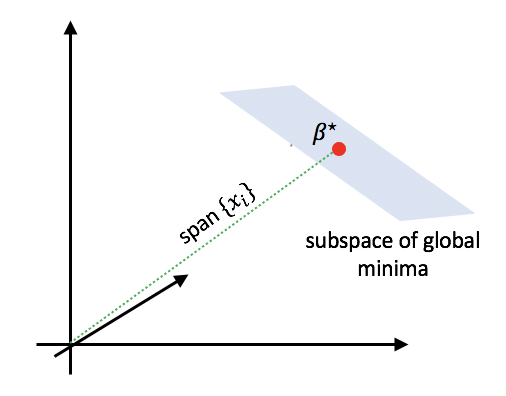
\includegraphics[width=.35\linewidth]{figures/subspace-global-min.png}
\caption{Visualization of proof intuition for Theorem~\ref{lec13:thm:linear-main}. The solution $\beta^\star$ is the projection of the origin onto the subspace of global minima.}
\label{lec13:fig:1}
\end{figure}

\begin{proof}
We first show via induction that $\beta^t \in \text{span}\l\{ x\sp{1}, \dots,x\sp{n} \r\}$ for all $t$. For the induction base case, note that $\beta^0 = 0 \in \text{span}\l\{ x\sp{1}, \dots,x\sp{n} \r\}$. Now suppose $\beta^{t-1} \in \text{span}\l\{ x\sp{1}, \dots,x\sp{n} \r\}$. Recall that $\beta^t = \beta^{t-1} - \eta \nabla \hatL(\beta^{t-1})$. Since left-multiplying any vector by $X^\top$ amounts to taking a linear combination of the rows of $X$, it follows that $\eta \nabla \hatL(\beta^{t-1}) = \eta X^\top(X\beta^{t-1} - y) \in \text{span}\l\{ x\sp{1}, \dots,x\sp{n} \r\}$, and so $\beta^t = \beta^{t-1} - \eta \nabla \hatL(\beta^{t-1}) \in \text{span}\l\{ x\sp{1}, \dots,x\sp{n} \r\}$. This proves the induction step.

Next, we show that $\hat \beta \in \text{span}\l\{ x\sp{1}, \dots,x\sp{n} \r\}$ and $\hatL(\hat \beta) = 0$ implies $\hat \beta = \beta^\star$. By definition, $\hat \beta \in \text{span}\l\{ x\sp{1}, \dots,x\sp{n} \r\}$ implies $\hat \beta = X^\top v$ for some $v \in \bbR^n$. Since $\hatL(\hat \beta) = 0$, we have $0 = X\hat \beta - y = X X^\top v - y$. This implies $v = (X X^\top)^{-1}y$, and so $\hat \beta = X^\top v = X^\top (X X^\top)^{-1} y = X^+ y = \hat \beta^\star$.
\end{proof}

\sec{Algorithmic regularization in non-linear models}
We give an example of algorithmic regularization in a non-convex version of the overparametrized linear regression task considered in the previous section.

Take $X$ and $y$ as defined in Section~\ref{lec13:sec:olr}. This time, our goal is to find a weight vector that minimizes our empirical loss function
\begin{equation}
\hatL(\beta) := \frac{1}{4n}\sum_{i=1}^n \left(y\sp{i} - f_\beta(x\sp{i})\right)^2,
\end{equation}
where $f_\beta(x):= \langle \beta \odot \beta, x\rangle$. (The operation $\odot$ denotes the Hadamard product: for $u,v \in \bbR^d$, $u \odot v \in \bbR^d$ is defined by $(u \odot v)_i := u_i v_i$ for $i = 1, \dots, d$.)

We assume $x\sp{1},...,x\sp{n} \iid \cN(0,I_{d \times d})$ and $y\sp{i} = f_{\beta^\star}(x\sp{i})$, where the ground truth vector $\beta^\star$ is $r$-sparse (i.e. $\|\beta^\star\|_0 = r$). For simplicity, we assume $\beta_i^\star = \mathbf{1} \{i \in S\}$ for some $S \subset [d]$ such that $|S| = r$. We again analyze the overparametrized setting, where this time $n \ll d$ but also $n \geq \widetilde \Omega(r^2)$.

\subsec{Main results of algorithmic regularization}
Note that while $f_\beta$ is still linear over $x$, our loss is no longer convex over $\beta$. (To see this, suppose $\beta \neq 0$ is a global minimizer. Then we have $\hatL(0) > \hatL(\beta) = \hatL(-\beta)$.) Thus, the effect of algorithmic regularization induced by gradient descent will be much different from the overparametrized linear regression setting. 

In the previous setting of linear regression, solutions with low $\ell_2$ norm are desirable as they tend to generalize well. In the present setting, we know our ground-truth parameter $\beta^\star$ is sparse. Thus, we want to learn a sparse solution $\hat \beta$, avoiding non-sparse solutions that may not generalize well. One approach to finding sparse solutions, called \textit{lasso regression}, is to minimize the $\ell_1$-regularized proxy loss
\begin{equation}
\sum_{i=1}^n \left(\langle \theta, x\sp{i} \rangle - y\sp{i} \right)^2 + \lambda \| \theta \|_1
\end{equation}
with respect to $\theta$, where $\theta = \beta \odot \beta$. However, it turns out that we can equivalently learn a sparse solution by running gradient descent from a suitable initialization on the original \textit{unregularized} loss.

To be specific, let $\beta^0=\alpha \mathbf{1} \in \R^d$ be the initialization where $\alpha$ is a small positive number. The update rule of gradient descent algorithm is given by $\beta^{t+1}=\beta^t-\eta\nabla \hatL(\beta^{t}).$ The next theorem shows that when $n=\widetilde{\Omega}(r^2)$, gradient descent on $\hatL(\beta)$ converges to $\beta^\star.$

\begin{theorem}\label{lec13:thm:non-linear-main}
Let $c$ be a sufficiently large universal constant. Suppose $n\ge cr^2\log^2(d)$ and $\alpha\le 1 / d^c$, then when $\dfrac{\log(d/\alpha)}{\eta}\lesssim T\lesssim \dfrac{1}{\eta\sqrt{d\alpha}},$ we have
\begin{equation}\label{lec13:eqn:non-linear-main}
    \l\|\beta^\top\odot\beta^\top-\beta^\star\odot\beta^\star \r\|_2^2\le O \l( \alpha\sqrt{d} \r).
\end{equation}

(Here, $T$ indexes the gradient descent steps.)
\end{theorem}

We make several remarks about Theorem~\ref{lec13:thm:non-linear-main} before presenting the proof.

\begin{remark}
In this problem we do not use $\beta^0=0$ as the initialization point because $\beta=0$ is a critical point, that is, $\nabla\hatL(0)=0$. Note that the lower bound on $T$ depends logarithimically on $1/\alpha$, so we can take $\alpha$ to be a small inverse polynomial on $d$ and the lower bound won't change much. Also, the upper bound depends polynomially on $1/\alpha$ (which is considered very big when $c$ is sufficiently large), so we do not need to use early stopping in a serious way.
\end{remark}

\begin{remark}
Theorem~\ref{lec13:thm:non-linear-main} is a simplified version of Theorem 1.1 in \cite{li2018algorithmic}.
\end{remark}

\begin{remark}
$\hatL(\beta)$ has many global minima. To see this, observe that the number of parameters is $d$ and the number of constraints to fit all the examples is $O(n)$ because there are only $n$ examples. Recall that for overparameterized model we have $d\gg n$; consequently, there exists many global minima of $\hatL(\beta)$.
\end{remark}

\begin{remark}
$\beta^\star$ is the min-norm solution in this case. That is,
    \begin{align}\label{lec13:eqn:opt}
        \beta^\star=\argmin \|\beta\|_2^2\qquad \text{s.t. }\hatL(\beta)=0.
    \end{align}
    Informally, this is because we can view $\beta\odot \beta$ as a vector $\theta\in \R^{d}$, which leads to $\|\beta\|_2^2 =\|\theta\|_1.$ Then in the $\theta$ space (and with a little abuse of notation), the optimization problem~\eqref{lec13:eqn:opt} becomes
    \begin{align}\label{lec13:eqn:opt-theta}
        \theta^\star=\argmin \|\theta\|_1 \qquad \text{s.t. }\hatL(\theta)=0,
    \end{align}
    which is a lasso regression, whose solution is sparse.
\end{remark}

\begin{remark}    
In this non-linear case and the linear case before, gradient descent with small initialization converges to minimum $\ell_2$-norm solution. Similarly, in the NTK regime, gradient descent converges to a solution that is very close to the initialization. Therefore, it seems conceivable that GD generally prefers global minima nearest to the initialization. However, we do not have a general theorem for this phenomenon (and the instructor also believes that this is not universally true without other conditions). 
\end{remark}

\subsec{Ground work for proof and the restricted isometry property}\label{lec13:sec:rip}

In this section we prepare the ground work for the proof of Theorem~\ref{lec13:thm:non-linear-main}.

We start by showing several basic properties about $\hatL(\beta)$. Note that for any fixed vector $v\in\R^{d}$ and $x\in \R^{d}$, when $x$ is drawn from $\cN(0,I)$, we have
\begin{equation}\label{lec13:eqn:gaussian-product}
    \Exp \l[\langle x, v\rangle^2 \r]=\Exp \l[ v^\top xx^\top v \r]=v^\top\Exp \l[ xx^\top \r]v=\|v\|_2^2.
\end{equation}

It follows that 
\begin{align}
    L(\beta)&=\frac{1}{4}\Exp_{x\sim \cN(0,I)} \l[(y-\langle \beta\odot\beta,x\rangle^2 \r] \\
    &=\frac{1}{4}\Exp_{x\sim \cN(0,I)} \l[\langle \beta^\star\odot\beta^\star-\beta\odot\beta,x\rangle^2 \r] &\text{(by definition of $y$)} \\
    &=\frac{1}{4} \l\| \beta^\star\odot\beta^\star-\beta\odot\beta \r\|_2^2.\label{lec13:eqn:loss-form} &\text{(by \eqref{lec13:eqn:gaussian-product})}
\end{align}
Note that \eqref{lec13:eqn:loss-form} is the metric that we use to characterize how close $\beta$ is to the ground-truch parameter $\beta^\star$ (see \eqref{lec13:eqn:non-linear-main}).

In the following lemma we show that $\hatL(\beta) \approx L(\beta)$ by uniform convergence. Generally speaking, uniform convergence of the loss function for all $\beta$ requires $n\ge \Omega(d)$ samples, so in our setting (where $n\ll d$) $\hatL(\beta) \approx L(\beta)$ does not always hold. However, since we assume $\beta^\star$ is sparse, the analysis only requires uniform convergence for sparse vectors.

\begin{lemma}\label{lec13:lem:RIP}
Assume $n\ge \widetilde\Omega(r^2)$. With high probability over the randomness in $x^{(1)},\cdots,x^{(n)}$, $\forall v$ such that $\|v\|_0\le r$ we have
\begin{equation}\label{lec13:eqn:RIP}
(1-\delta)\|v\|_2^2\le \frac{1}{n}\sum_{i=1}^{n}\langle v,x^{(i)}\rangle^2\le (1+\delta)\|v\|_2^2.
\end{equation}
\end{lemma}

Lemma~\ref{lec13:lem:RIP} is a special case of Lemma 2.2 in \cite{li2018algorithmic} so the proof is omitted here. We say the set $\l\{ x^{(1)},\cdots,x^{(n)} \r\}$ (or $X=[x^{(1)},\cdots,x^{(n)}]$) satisfies $(r,\delta)$\textit{-RIP condition} (\textit{restricted isometric property}) if \eqref{lec13:eqn:RIP} holds.

By algebraic manipulation, \eqref{lec13:eqn:RIP} is equivalent to 
\begin{align}\label{lec13:eqn:RIP-2}
(1-\delta)\|v\|_2^2\le v^\top \left(\frac{1}{n}\sum_{i=1}^{n}x^{(i)}(x^{(i)})^\top\right)v\le (1+\delta)\|v\|_2^2.
\end{align}
In other words, from the point of view of a sparse vector $v$ we have $\sum_{i=1}^{n}x^{(i)}(x^{(i)})^\top\approx I$. (Note however that $\sum_{i=1}^{n}x^{(i)}(x^{(i)})^\top$ is not close to $I_{d\times d}$ in other notions of closeness. For example, $\sum_{i=1}^{n}x^{(i)}(x^{(i)})^\top$ is not close to $I_{d\times d}$ in spectral norm. Another way to see this is that $\sum_{i=1}^{n}x^{(i)}(x^{(i)})^\top$ is a $d \times d$ matrix but only has rank $n \ll d$.)

As a result, with the RIP condition we have $\hatL(\beta)\approx L(\beta)$ if $\beta$ is sparse. With more tools we can also get $\nabla \hatL(\beta)\approx \nabla L(\beta)$. Let us define the set $S_r=\{\beta:\|\beta\|_0\le O(r)\}$, the set where we have uniform convergence of $\hatL$ and $\nabla \hatL$. Informally, as long as we are in the set $S_r$, $\hatL$ and $\nabla\hatL$ have similar behavior to their population counterparts. (Note, on the other hand, that there exists a dense $\beta\not\in S_r$ such that $\hatL(\beta)=0$ but $L(\beta)\gg 0.$)

The RIP condition also gives us the following lemma which will be needed for the proof of Theorem \ref{lec13:thm:non-linear-main}.

\begin{lemma}\label{lec14:lem:rip}
    Suppose $x^{(1)}, x^{(2)}, \dots x^{(n)}$ satisfy the $(r, \delta)$-RIP condition. Then, $\forall v, w$ such that $\Norm{v}_{0} \leq r$ and $\Norm{w}_{0} \leq r$, we have that
    \begin{align}
        \left| \frac{1}{n} \sum_{i=1}^{n} \langle x^{(i)}, v \rangle \langle x^{(i)}, w \rangle  - \langle v, w \rangle \right| &= \left|  v^{T} \l(\frac{1}{n} \sum_{i=1}^{n}  x^{(i)} (x^{(i)})^\top \r)  w  - \langle v, w \rangle \right| \\
        &\leq 4 \delta \Norm{v}_{2} \cdot \Norm{w}_{2}.
    \end{align} 
\end{lemma}

\tnotelong{To add proof of this lemma in the future.}
\begin{corollary}\label{lec14:cor:rip}
    Taking $w = e_1, \dots, e_d$ in Lemma~\ref{lec14:lem:rip}, we can conclude that
    \begin{align}
        \Norm{ \frac{1}{n} \sum_{i=1}^n \langle x^{(i)}, v\rangle x^{(i)} - v }_\infty &= \Norm{ \l(\frac{1}{n} \sum_{i=1}^n x^{(i)}(x^{(i)})^\top \r)v - v }_\infty \\
        &\leq 4\delta \Norm{v}_2.
    \end{align}
\end{corollary}

\subsec{Warm up: Gradient descent on population loss}

The main intuition for proving Theorem~\ref{lec13:thm:non-linear-main} is to leverage the uniform convergence when $\beta$ belongs to the set $S_r$ (see Figure~\ref{lec13:fig:uc-sr}). Note that the initialization $\beta^0$ is not exactly $r$-sparse, but taking $\alpha$ to be sufficiently small, $\beta^0$ is approximately $0$-sparse. The proof is decomposed into the following steps:

\begin{enumerate}
    \item Gradient descent on $L(\beta)$ converges to $\beta^\star$ without leaving $S_r$, and
    \item Gradient descent on $\hatL(\beta)$ is similar to gradient descent on $L(\beta)$ inside $S_r$.
\end{enumerate}

Combining the two steps we can show that gradient descent on $\hatL(\beta)$ does not leave $S_r$ and converges to $\beta^\star.$

\begin{figure}
\centering
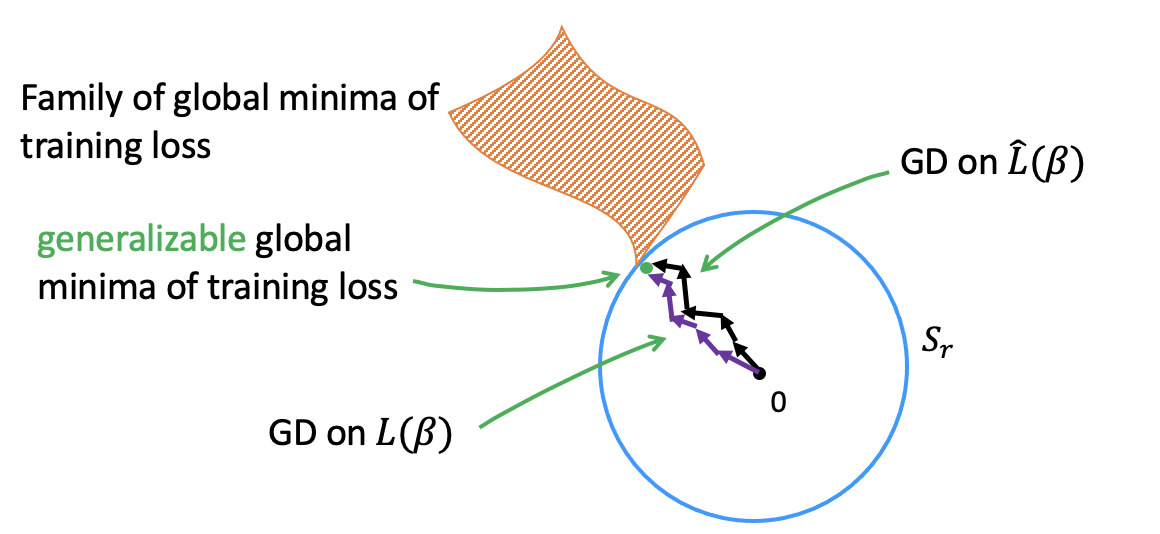
\includegraphics[width=.7\linewidth]{figures/uc-sr.png}
\caption{Visualization of proof intuition for Theorem~\ref{lec13:thm:non-linear-main}.}
\label{lec13:fig:uc-sr}
\end{figure}

As a warm up, we prove the following theorem for gradient descent on $L(\beta).$
\begin{theorem}
For sufficiently small $\eta$, gradient descent on $L(\beta)$ converges to $\beta^\star$ in $\Theta\left(\dfrac{\log (1/ (\epsilon\alpha) )}{\eta}\right)$ iteration with $\epsilon$-error in $\ell_2$-distance.
\end{theorem}

\begin{proof}

Since
\begin{equation}
\nabla L(\beta) = (\beta\odot \beta-\beta^\star\odot\beta^\star)\odot\beta,
\end{equation}

the gradient descent step is
\begin{equation}
\beta^{t+1} = \beta^t - \eta (\beta^t \odot \beta^t -\beta^\star \odot \beta^\star)\odot\beta^t.
\end{equation}

Recall that $\beta^\star=\mathbf{1} \{i \in S \}$ and $\beta^0=\alpha \mathbf{1}$, and the update rule above decouples across the coordinates of $\beta^t$. Thus, we only need to show that $| \beta_i^\star - \beta^t | \leq \epsilon$ for the number of iterations stated in the Theorem.

\underline{Case 1: $i\in S$.} For $i \in S$, the update rule for coordinate $i$ is
\begin{align}
\beta_i^{t+1} &= \beta_i^t - \eta (\beta_i^t \cdot \beta_i^t - 1 \cdot 1) \cdot\beta_i^t \\ 
&= \beta_i^t - \eta \l[ \left(\beta_i^t\right)^2 - 1 \r] \beta_i^t.
\end{align}

Consider the following two cases:

\begin{itemize}
\item If $\beta_i^t\le 1/2$, we have
\begin{align}
\beta_i^{t+1}&=\beta_i^{t} \l[ 1+\eta \l(1- \l(\beta_i^t \r)^2 \r) \r] \\
&\ge \beta_i^t \l( 1+\frac{3}{4}\eta \r).
\end{align}

Consequently, $\beta_i^{t+1}$ grow exponentially, and it takes $\Theta\left(\dfrac{\log (1/\alpha)}{\eta}\right)$ iterations for $\beta_i^t$ to grow from $\alpha$ to at least $1/2.$\footnote{This is because $(1+\eta)^{1/\eta}\approx e$, so $(1+\eta)^{c/\eta}\approx e^{c}.$} This will bring us into the second case.
    
\item if $\beta_i^t\ge 1/2$, we have
\begin{align}
1-\beta_i^{t+1}&=1-\beta_i^t+\eta \l[ \l(\beta_i^t \r)^2-1 \r] \beta_i^t\\
&=1-\beta_i^{t}-\eta \l( 1-\beta_i^t \r) \l(1+\beta_i^t \r)\beta_i^t\\
&\le 1-\beta_i^t-\eta \l( 1-\beta_i^t \r)\beta_i^t &\text{(because $1+\beta_i^t\ge 1$)} \\
&= \l(1-\beta_i^t \r) \l( 1-\eta \beta_i^t \r) \\
&\le \l( 1-\beta_i^t \r) \l(1-\eta/2 \r). &\text{(because $\beta_i^t\ge 1/2$)}
\end{align}

Therefore it takes $\Theta\left(\dfrac{\log (1/\epsilon)}{\eta}\right)$ iterations to achieve $1-\beta_i^t\le \epsilon.$
\end{itemize}

\underline{Case 2: $i \notin S$.} For all $i \notin S$, we claim (informally) that it is sufficient to show that when $t \leq 1 / (10 \eta \alpha^{2})$, $\beta_{i}^{t} \leq 2\alpha$. This is because when $i \notin S$, $\beta_{i}$ stays small and will take many iterations before it even gets to $2\alpha$, which is close to $0$ since $\alpha$ is chosen to be small.

For a coordinate $i\notin S$, the gradient descent update for this problem becomes
\begin{align}
    \beta_i^{t+1} &= \left[ \beta^{t} - \eta (\beta^{t} \odot \beta^{t} - \beta^\star \odot \beta^\star) \odot \beta^{t} \right]_i \\
    &= \beta_i^{t} - \eta (\beta_i^{t} \cdot \beta_i^{t}) \cdot \beta_i^{t} & (\text{since } \beta_{i}^\star = 0 \ \forall i \notin S) \\
    &= \beta_i^{t} - \eta (\beta_i^{t})^{3}.
\end{align}

Since our initialization $\beta^{0}$ was small, the update to these coordinates will be even smaller because $(\beta_{i}^{t})^{3}$ is small. We can prove the desired claim using strong induction. Suppose $\beta_{i}^{s} \leq 2\alpha$ for all $s \leq t$ and $i \notin S$, and that $t+1 \leq 1 / (10\eta \alpha^{2})$. Then, for all $s \leq t$,
\begin{align}
\beta_{i}^{s+1} %&= \beta^{s}_{i} - \eta (\beta_{i}^{s})^{3} \\
    &= (1 - \eta (\beta_{i}^{s})^{2})\beta_{i}^{s} \\
    &\leq (1 + \eta (\beta_{i}^{s})^{2}) \beta_{i}^{s} \\
    &\leq (1 + 4\eta \alpha^{2}) \beta_{i}^{s}. & (\text{since } \beta_{i}^{s} \leq 2\alpha)
\end{align}

With strong induction, we can repeatedly apply this gradient update starting from $t=0$ to obtain
\begin{align}
    \beta_{i}^{t+1} &\leq \beta_{0} \cdot (1 + 4 \eta \alpha^{2})^t \\
    &\leq \beta_{0} ( 1 + 4 \eta \alpha^{2})^{\frac{1}{10 \eta \alpha^{2} }} \\
    &\leq \beta_{0} \exp \bigg(\frac{4\eta \alpha^{2}}{10 \eta \alpha^{2}} \bigg) \\
    &=  \beta_{0} \cdot e^{2/5} \\
    &\leq 2 \alpha,
 \end{align}
 which completes the inductive proof of the claim.

\end{proof}